\ifx\mainfile\undefined
%  ========================================================================
%  Copyright (c) 2006-2011 The University of Washington
%
%  Licensed under the Apache License, Version 2.0 (the "License");
%  you may not use this file except in compliance with the License.
%  You may obtain a copy of the License at
%
%      http://www.apache.org/licenses/LICENSE-2.0
%
%  Unless required by applicable law or agreed to in writing, software
%  distributed under the License is distributed on an "AS IS" BASIS,
%  WITHOUT WARRANTIES OR CONDITIONS OF ANY KIND, either express or implied.
%  See the License for the specific language governing permissions and
%  limitations under the License.
%  ========================================================================
%
 
\documentclass [11pt, twoside] {uwthesis}

\usepackage{color}
\usepackage{url}
\usepackage{amsmath}
\usepackage{amsfonts}
\usepackage[bookmarks,
	hidelinks,
	plainpages=false,
	pdfpagelabels,
	pagebackref=true,
            ]{hyperref}
\renewcommand*{\backref}[1]{}% for backref < 1.33 necessary
\renewcommand*{\backrefalt}[4]{%
  \ifcase #1 %
    (No citations.)%
  \or
    (Cited on page #2.)%
  \else
    (Cited on pages #2.)%
  \fi
}

\newcommand{\biburl}[1]{{\tt<}\url{#1}{\tt>}}

\hypersetup{%
pdfauthor = {Daniel Chaim Halperin},
pdftitle = {Simplifying the Configuration of 802.11 Wireless Networks with Effective SNR},
pdfsubject = {Ph.D. Dissertation},
pdfkeywords = {},
pdfcreator = {University of Washington, Computer Science and Engineering},
pdfproducer = {},
bookmarksopen = {true},
pdfpagelayout = {TwoColumnRight},
}

\usepackage{footnotebackref}
%%%%%%%%%%%%%%%%%%%%%%%%%%%%%%%%%%%%%%%%%%%%%%%%%%%%%%
%%%        Formatting sections                     %%%
%%%%%%%%%%%%%%%%%%%%%%%%%%%%%%%%%%%%%%%%%%%%%%%%%%%%%%
\newcommand{\algref}[1]{Algorithm~\ref{#1}}
\newcommand{\chapref}[1]{Chapter~\ref{#1}}
\renewcommand{\eqref}[1]{Equation~\ref{#1}}
\newcommand{\figref}[1]{Figure~\ref{#1}}
\newcommand{\secref}[1]{\S\ref{#1}}
\newcommand{\tabref}[1]{Table~\ref{#1}}
\newcommand{\heading}[1]{\vspace{4pt}\noindent\textbf{#1}}
\newcommand{\topheading}[1]{\noindent\textbf{#1}}
\newcommand{\noheading}[0]{\vspace{4pt}\noindent}

%%%%%%%%%%%%%%%%%%%%%%%%%%%%%%%%%%%%%%%%%%%%%%%%%%%%%%
%%%        XXX and other warnings                  %%%
%%%%%%%%%%%%%%%%%%%%%%%%%%%%%%%%%%%%%%%%%%%%%%%%%%%%%%
\newcommand{\xxx}[1]{\textit{\color{red}XXX #1}}

%%%%%%%%%%%%%%%%%%%%%%%%%%%%%%%%%%%%%%%%%%%%%%%%%%%%%%
%%%        Units                                   %%%
%%%%%%%%%%%%%%%%%%%%%%%%%%%%%%%%%%%%%%%%%%%%%%%%%%%%%%
\usepackage{xspace}
\newcommand{\unitsep}{\texorpdfstring{\,}{ }}
\def\unit#1{% from: http://www.tex.ac.uk/cgi-bin/texfaq2html?label=csname "Defining a macro from an argument"
  \expandafter\def\csname #1\endcsname{\unitsep\text{#1}\xspace}%
}
\def\varunit#1#2{% from: http://www.tex.ac.uk/cgi-bin/texfaq2html?label=csname "Defining a macro from an argument"
  \expandafter\def\csname #1\endcsname{\unitsep\text{#2}\xspace}%
}
\unit{GHz}
\unit{MHz}
\unit{kHz}
\unit{Gbps}
\unit{Mbps}
\unit{KB}
\unit{dB}
\unit{dBi}
\unit{dBm}
\unit{W}
\unit{mW}
\varunit{uW}{$\mu$W}
\unit{ms}
\varunit{us}{$\mu$s}
\unit{h}
\unit{m}
\unit{s}
\unit{km}
\unit{cm}
\unit{mm}
\varunit{mmsq}{mm$^\text{2}$}
\varunit{insq}{in$^\text{2}$}
\newcommand{\degree}{\ensuremath{^\circ}\xspace}
\newcommand{\degrees}{\degree}
%%%%%%%%%%%%%%%%%%%%%%%%%%%%%%%%%%%%%%%%%%%%%%%%%%%%%%%%%%%%%%%%%%%%%%%%%%%%%%%%%%%%%%
% Euler for math | Palatino for rm | Helvetica for ss | Courier for tt
%
% From: http://www.tug.org/mactex/fonts/LaTeX_Preamble-Font_Choices.html
%%%%%%%%%%%%%%%%%%%%%%%%%%%%%%%%%%%%%%%%%%%%%%%%%%%%%%%%%%%%%%%%%%%%%%%%%%%%%%%%%%%%%%
\renewcommand{\rmdefault}{ppl} % rm
\usepackage[scaled]{helvet} % ss
\usepackage{courier} % tt
\usepackage{eulervm} % a better implementation of the euler package (not in gwTeX)
\normalfont
\usepackage[T1]{fontenc}
%%%%%%%%%%%%%%%%%%%%%%%%%%%%%%%%%%%%%%%%%%%%%%%%%%%%%%%%%%%%%%%%%%%%%%%%%%%%%%%%%%%%%%

%%%%%%%%%%%%%%%%%%%%%%%%%%%%%%%%%%%%%%%%%%%%%%%%%%%%%%
%%%        Figures                                 %%%
%%%%%%%%%%%%%%%%%%%%%%%%%%%%%%%%%%%%%%%%%%%%%%%%%%%%%%
\usepackage{graphicx}
% Caption package both lets you set the spacing between figure and caption
% and also makes the \figref{} point to the right place.
\usepackage[font=bf,aboveskip=6pt,belowskip=-4mm]{caption}
% Allow subfigures, make them bold
\usepackage[bf,BF,small]{subfigure}
% List of figures
\setcounter{lofdepth}{2}  % Print the chapter and sections to the lot

%%%%%%%%%%%%%%%%%%%%%%%%%%%%%%%%%%%%%%%%%%%%%%%%%%%%%%
%%%        Lists with reduced spacing              %%%
%%%%%%%%%%%%%%%%%%%%%%%%%%%%%%%%%%%%%%%%%%%%%%%%%%%%%%
\usepackage{enumitem}

%%%%%%%%%%%%%%%%%%%%%%%%%%%%%%%%%%%%%%%%%%%%%%%%%%%%%%
%%%        Fancy tables                            %%%
%%%%%%%%%%%%%%%%%%%%%%%%%%%%%%%%%%%%%%%%%%%%%%%%%%%%%%
\usepackage{tabulary}
\usepackage{booktabs}

%%%%%%%%%%%%%%%%%%%%%%%%%%%%%%%%%%%%%%%%%%%%%%%%%%%%%%
%%%        Formatting techniques/tools/etc.        %%%
%%%%%%%%%%%%%%%%%%%%%%%%%%%%%%%%%%%%%%%%%%%%%%%%%%%%%%
\newcommand{\term}[1]{\texttt{#1}}

\begin{document}
 
\textpages
\setcounter{chapter}{4} % Set to n-1!
\fi
%%%%%%%%%%%%%%%%%%%%%%%%%%%%%%%%%%

\cleardoublepage
\chapter{Measuring 802.11n Traces with Channel State Information}
\label{chap:esnr_intro}

In this section, we describe our preliminary work building an experimental 802.11n platform, in particular a tool that uses commodity Intel Wi-FI NICs to measure the 802.11n Channel State Information. Next, we use measurements of packet delivery vs RSSI and CSI to show explain why RSSI fails to predict packet delivery in real wireless channels. When then use CSI in conjunction with the concept of an Effective SNR for wireless links to explain the performance of links that experience frequency-selective fading. We demonstrate experimentally that CSI and Effective SNR can predict the performance of wireless links across a wide range of configurations, such as rate selection and transmit power control. Finally, we present trace-driven simulation results that show that a simple Effective SNR-based rate \emph{selection} (not \emph{adaptation}) can be used to achieve good performance in varying channels.

\section{802.11n CSI Tool and Experimental Platform}
\label{sec:platform}
In conjunction with Intel Labs Seattle, we have built an experimental 802.11n platform that uses the Intel Wi-Fi Wireless Link 5300 (\term{iwl5300}) 802.11a/b/g/n network cards. We modified the closed-source firmware and open-source Linux driver to add a number of experimental features importantly to measure the 802.11n CSI\@. Here, we summarize these features.

\heading{802.11n CSI Measurement.} The channel sounding mechanism added in 802.11n defines a management frame used to report the CSI from the receiver of a frame back to the transmitter. This mechanism is intended for calibration or to inform transmit beamforming, and we co-opt it for our experiments. We configure the NIC with a debug mode to compute this feedback packet for every received frame,\footnote{CSI is reported for correctly received frames destined for the measurement node or sent to a special hard-coded broadcast address.} rather than just during sounding, and send it up to the driver instead of back to the transmitter. The \term{iwl5300} provides CSI in a format that reports the channel matrices for 30 subcarrier groups, which is about one group for every 2 subcarriers at 20\MHz or every 4 subcarriers at 40\MHz. Each channel matrix entry is a complex number, with signed 8-bit resolution each for the real and imaginary parts. It specifies the gain and phase of the spatial path between a single transmit-receive antenna pair. Intel's implementation of the 802.11n CSI does not include per-subcarrier noise measurements, so we assume the noise floor is uniform across all subcarriers to compute SNRs. This is consistent with white noise observed on other OFDM platforms~\cite{Rahul_FARA}.

\heading{RSSI Measurement.} 
For each received packet the NIC reports the traditional metrics of RSSI per receive antenna, noise floor and the setting on the automatic gain controlled (AGC) amplifier. These combine to define the per-receive-chain packet SNR ($\rho_{\text{packet}}$):
\begin{equation}
\label{eq:per_chain_snr}
	\rho_{\text{packet}} = \text{RSSI (dBm)} - \text{Noise (dBm)} - \text{AGC (dB)}
\end{equation}
The \term{iwl5300} calculates the quantities RSSI and Noise as the respective sums of average signal strength and average error vector magnitude in each OFDM subcarrier~\cite{iwlwifi}. This is exactly the traditional definition of SNR applied to OFDM\@.

\heading{Transmit Power Control.} Our hardware enables us to vary the transmit power level from $-$10\dBm~(100\uW) to $+$16\dBm~(40\mW) in steps of 0.5\dB, and divides power equally across streams. Additionally, the \term{iwl5300} reduces the transmit power slightly when using the highest single-stream rates to avoid distortions caused by passing QAM-64 symbols with high peak-to-average power ratio through the transmit amplifier.

\heading{Rapid Rate Variation.} In normal operation, the \term{iwl5300} decouples queuing packets for transmission from selecting rates for these packets, since queues must be kept large to take advantage of 802.11n block transmissions. This makes it difficult to control the rate at which individual packets are transmitted. We modified the firmware and driver to support the transmission of individual packets at predetermined rates, and added driver-level code to rapidly iterate through a user-configurable set of available rates.

\heading{Userspace Connector.} We used the Linux kernel \term{connector} framework to implement a low-latency socket-based communication channel between the kernel driver and userspace utilities. This enables userspace utilities to logging of CSI and other output from the driver, and send messages that, e.g., change the currently selected rate or antennas or change the transmit power level.

\heading{Publicly Released Tool.} We have publicly released our experimental platform and CSI collection tool in the form of open source drivers, userspace utilities, MATLAB code, and binary firmware image~\cite{Halperin_csitool}. At the time of writing, we are aware of several users, including multiple research and product groups within Intel, industrial researchers at HP Labs, and academic researchers at UT Austin, CMU, UCL, and the Hong Kong University of Science and Technology.

\begin{figure}[t]
  \centering
  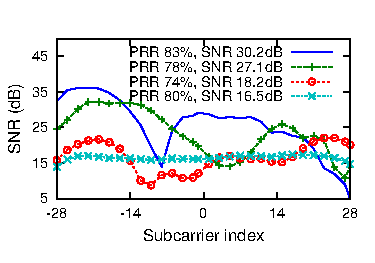
\includegraphics[width=\columnwidth,viewport=2 9 185 108,clip]{figures/esnr/embed_fsf-shape-two-links.pdf}
% viewport=2 10 170 108
  \caption{Channel gains on four links that perform about equally well at 52\Mbps. The more faded links require larger RSSIs (i.e., more transmit power) to achieve similar PRRs.}
  \label{fig:example_fsf_shape}
  % information for the links used to make above plot: 
  %srcs = [1 10 3 3];
  %dests = [9 11 2 5];
  %txpowers = [-4 20 28 20];

  % reference numbers from expt-8
  %prr = [80 83 78 74];
  %rss = [16.5 30.2 27.1 18.2];
\end{figure}

\heading{Example: RSSI vs CSI\@.}
To contrast CSI and RSSI, \figref{fig:example_fsf_shape} shows packet delivery rates, RSSIs, and subcarrier-level CSI for four links that exhibit similar performance when using the 802.11n single-stream 52\Mbps rate. Multipath causes some subcarriers to work markedly better than others although all use the same modulation and coding. These channel details, and not simply the overall signal strength as given by RSSI, affect packet delivery. The fading profiles vary significantly across the four links. One distribution is quite flat across the subcarriers, while the other three exhibit frequency-selective fading of varying degrees. Two of the links have two deeply-faded subcarriers that are more than 20\dB down from the peak.

These links harness the received power with different efficiencies.
The more faded links are more likely to have errors that must be repaired with coding, and require extra transmit power to compensate. Thus, while the performance is roughly the same, the most frequency-selective link needs a much higher overall packet SNR~(30.2\dB) than the frequency-flat link (16.5\dB). This difference of almost 14\dB highlights why RSSI-based SNR does not reliably predict performance. Fading and its effects are well-known. However, it is rare to see data that shows fading for real links and NICs because it has been difficult to measure.

\section{Effective SNR Model for 802.11n}
The example of \figref{fig:example_fsf_shape} indicated that the extra information in CSI can help explain performance for real wireless links. Here, we develop a model that can accurately predict the packet delivery probability of commodity 802.11 NICs for a given physical layer configuration operating over a given channel. We want our model to be simple and practical, so that it can be readily deployed, and to cover a wide range of physical layer configurations, so that it can be applied in many settings and for many tasks. In particular, the scope of our model is 802.11n including multiple antenna modes, including OFDM and MIMO\@. This scope is sufficient for many current and future networks. In our preliminary work, we have modeled delivery for single packet transmission only.

\heading{Model Design.}
The structure of our model is simple: given 1) a current CSI measurement of the RF channel between transmitter and receiver, and 2) a target physical layer configuration of the transmit and receive NICs, it predicts whether that link will reliably deliver packets in that configuration.
With this simple decision primitive, we can easily build higher layer optimization protocols. These include selecting the best rate, number of spatial streams, or transmit antenna set; whether to use 20\MHz or the entire 40\MHz channel; or choosing the lowest transmit power at which the link supports a particular rate.

For the model output, we define that the link will work, i.e., will reliably deliver packets, if we predict $\geq$90\% packet reception rate. We do not try to make predictions in the transition region during which a link changes from lossy to reliable. Predictions there are likely to be variable, and simply knowing when the link starts to work is useful information in practice.

%%%%%%%%%%%%%%%%%%%%%%%%%%%%%%%%%%
\ifx\mainfile\undefined
%
% ==========   Bibliography   ==========
%
%\nocite{*}   % include everything in the uwthesis.bib file
\bibliographystyle{plain}
\bibliography{dhalperi_thesis}

\end{document}
\fi